% Both source strokes run left to right. The first rectangle is written
% northeast to southwest; the second is written southeast to northwest.
% Blue survives from (0.5,1.1) to (2.4,1.86); red from (1,-0.45) to
% (3.5,0.05). The teal end caps join these independent pairs of endpoints.
\documentclass[border=2pt]{standalone}
\usepackage{pgfplots}
\usepgfplotslibrary{fillbetween}
\pgfplotsset{compat=1.18}
\begin{document}
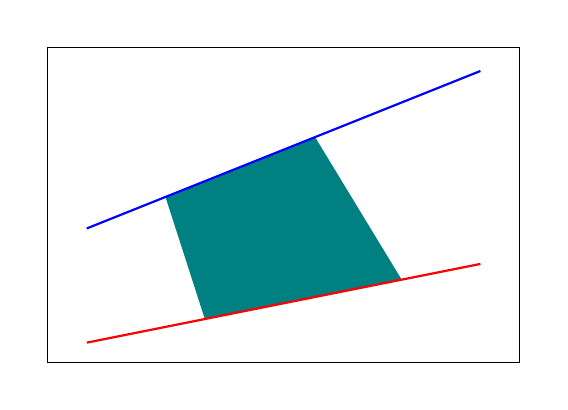
\begin{tikzpicture}
  \begin{axis}[at={(0,0)},anchor=south west,width=6cm,height=4cm,scale only axis,
    xmin=-1,xmax=5,ymin=-1,ymax=3,enlargelimits=false,axis lines=box,ticks=none]
    \addplot[blue,thick,mark=none,name path=upper] coordinates {(-0.5,0.7) (4.5,2.7)};
    \addplot[red,thick,mark=none,name path=lower] coordinates {(-0.5,-0.75) (4.5,0.25)};
    \addplot[draw=none,fill=teal] fill between[of=upper and lower,
      soft clip first={(axis cs:2.4,2.4) rectangle (axis cs:-0.3,1.1)},
      soft clip second={(axis cs:4.3,-0.55) rectangle (axis cs:1,0.05)}];
  \end{axis}
  \path[use as bounding box] (-0.25,-0.25) rectangle (6.25,4.25);
\end{tikzpicture}
\end{document}
